\documentclass[UTF8,zihao=-4]{ctexart}
\usepackage[a4paper,margin=2.30cm]{geometry}
\usepackage{amsmath,amssymb,amsthm,mathtools,bm}
\usepackage{booktabs,array}
\usepackage{graphicx}
\usepackage{float}
\usepackage{caption}
\usepackage{microtype}
\usepackage{enumitem}
\usepackage{etoolbox}
\usepackage[hidelinks]{hyperref}
\usepackage{url}

\AtBeginEnvironment{thebibliography}{\small}
\AtBeginEnvironment{abstract}{\small}

\captionsetup{font=small,labelfont=bf,skip=3pt}
\setlength{\parindent}{2em}
\setlength{\parskip}{0.12em}
\setlength{\abovedisplayskip}{5pt plus 1pt minus 1pt}
\setlength{\belowdisplayskip}{5pt plus 1pt minus 1pt}
\setlength{\abovedisplayshortskip}{2pt}
\setlength{\belowdisplayshortskip}{3pt}
\setlist{nosep,leftmargin=2.2em}
\setlength{\emergencystretch}{2.5em}
\renewcommand{\topfraction}{0.9}
\renewcommand{\bottomfraction}{0.6}
\renewcommand{\textfraction}{0.08}
\renewcommand{\floatpagefraction}{0.7}

\newtheorem{proposition}{命题}
\theoremstyle{remark}
\newtheorem{remark}{注}

\title{基于持续同调的变点检验：重叠滑动窗口下的\\[-6pt]有限样本校准\\[4pt]
\large Finite-Sample Calibration of Persistent-Homology-Based Change-Point Tests with Overlapping Windows}
\author{
  王平\textsuperscript{1}\quad
  黄盛南\textsuperscript{1}\quad
  张晓媛\textsuperscript{1,*}\\[1mm]
  \small $^1$河北金融学院统计与数据科学学院\quad
  通讯作者：张晓媛，\texttt{zxy0407010229@163.com}
}
\date{}

\hypersetup{
  pdftitle={基于持续同调的变点检验：重叠滑动窗口下的有限样本校准},
  pdfauthor={王平, 黄盛南, 张晓媛},
  pdfsubject={Finite-sample calibration of persistent-homology change-point tests with overlapping windows}
}

\begin{document}
\maketitle
\vspace{-2.4em}

{\footnotesize
\noindent\textbf{摘要}\quad
滑动窗口可用于提取时间序列的局部持续同调特征；窗口共享观测可能引入特征依赖，使随机置换所依据的联合交换性失效。本文评价“固定持续图向量表示＋最大扫描”检验的有限样本校准：先以窗口均值反例说明原始观测独立同分布不足以保证窗口序列可交换，再在固定窗口数与固定观测长度两种预算下，于 28 个零假设配置比较无约束窗口级置换（M0）与依赖乘子自助法（M1），并以均值—协方差特征（MOMENTS）作非拓扑对照。名义水平 0.05 下，两种表示的 20 个重叠配置 M0 均实质反保守（持续同调表示最高拒绝率 0.9756）；M1 在全部 56 个匹配组合中降低拒绝率，但 8 个非重叠配置均实质保守，未实现统一校准。三项预设对比（两数据生成过程等权平均）分别是重叠—非重叠 M0 拒绝率差与固定窗口数非重叠端的 M1 保守偏差，估计为 0.5354、0.5330 与 0.0266。圆到八字形的矩匹配备择下，尺寸校正功效为 1.00000 与 0.06203；整体平移负对照呈相反次序，与欧氏持续同调的平移不变性一致。降低拒绝率不等于恢复名义水平，敏感性与误报控制应分别评价。

\noindent\textbf{关键词}：持续同调；变点检测；重叠滑动窗口；交换性；有限样本校准

\par}

\vspace{0.2em}
{\footnotesize
\noindent\textbf{Abstract.}\quad
Sliding windows provide persistent-homology features, but shared observations can induce dependence and invalidate the exchangeability underlying window-level random permutation. This study evaluates the finite-sample calibration of a change-point test combining a fixed persistence-diagram representation (BPI) with a maximum scan statistic. A window-mean counterexample shows that i.i.d.\ raw observations need not yield exchangeable window features. Unrestricted window-level permutation (M0) and a dependent multiplier bootstrap (M1) are compared across 28 null configurations under fixed-window-count and fixed-observation-length designs, with mean--covariance features (MOMENTS) as a comparator. At the nominal level of 0.05, M0 is materially anti-conservative in all 20 overlapping configurations for each representation; the BPI rejection rate reaches 0.9756. M1 lowers rejection rates in all 56 matched configuration--representation combinations, yet is materially conservative in all eight non-overlapping configurations for each representation. For BPI with i.i.d.\ raw observations, equal averaging over the two generators yields M0 rejection-rate differences between strides 16 and 64 of 0.5354 and 0.5330 under the two designs. With 192 non-overlapping windows, the M1 rejection-rate deficit relative to 0.05 is 0.0266. Under a circle-to-figure-eight alternative with matched first and second marginal moments, size-adjusted powers are 1.0000 for BPI and 0.0620 for MOMENTS. A mean-shift negative control reverses the ordering, consistent with the translation invariance of persistent homology from Euclidean distances. Calibration is therefore condition-dependent for the studied implementation: lower rejection rates do not necessarily imply nominal calibration, and representation sensitivity and Type-I error control require separate evaluation.

\noindent\textbf{Keywords}: persistent homology; change-point detection; overlapping sliding windows; exchangeability; finite-sample calibration
\par}

\section{引言}\label{sec:intro}

时间序列的结构变化既可能表现为均值、方差等低阶统计量的改变，也可能表现为局部轨迹几何、周期结构或状态空间形状的改变。滑动窗口把每个时间片段映射为点云，持续同调再从多尺度上提取连通分支与环，为后一类信号提供局部化表示\mcite{PereaHarer2015,Adams2017}；拓扑摘要已用于离线检测、在线监测与依赖序列中的结构异常识别\mcite{IslambekovYuvarajGel2020,ZhengMakXieXie2023,ChazalLevrardRoyer2024,NieYue2026}。为提高候选点密度，实践常取步长 $s<W$，相邻窗口因而共享原始观测，窗口特征序列随之形成局部依赖。

已有工作利用持续同调开展离线变点检测或在线监测；文献\cite{NieYue2026}进一步给出局部窗口映射的依赖继承结果并进行块校准。本文固定持续图向量表示与离线最大扫描，在两种观测预算下比较指定置换和依赖乘子规则的有限样本拒绝率，关注其逐条件偏差。

推断层面的困难来自随机化单位与科学零假设的层级错配。设第 $i$ 个窗口经固定映射得到特征 $Y_i$。无约束随机置换获得有限样本水平控制的常用理论依据，是窗口特征的联合分布对所用排列群保持不变：
\begin{equation}\label{eq:exchangeability}
 (Y_1,\ldots,Y_M)\overset{d}{=}(Y_{\pi(1)},\ldots,Y_{\pi(M)}),
 \qquad \forall\,\pi\in\mathfrak S_M .
\end{equation}
若窗口特征序列本身独立同分布，则式\eqref{eq:exchangeability}成立；原始观测的独立同分布性质不能在窗口重叠时自动传递为窗口特征的交换性。平稳性与相同边际分布也不足以一般地推出该联合对称性\mcite{RomanoTirlea2022,HemerikGoeman2018}。科学零假设定义在原始过程的“无变化”层面，置换参考分布所需的对称性则定义在派生特征的联合分布层面，二者并不自动一致。

本文评价一种固定实现：窗口点云经持续同调与固定向量化得到 800 维表示（BPI），或经均值—协方差得到低维表示（MOMENTS），再以标准化部分和的最大值作扫描检验，分别用无约束窗口级置换（M0）与依赖乘子自助法（M1）校准。本文在预设设计域内比较两种校准方法的有限样本表现，报告 28 个配置、112 个“配置—表示—方法”单元的拒绝率、Wilson 分类及三项预设对比；窗口均值反例与两类构造备择分别用于解释交换性风险和表示敏感性。本文不给出 BPI 扫描的通用有限样本定理，全部结论限定于所考察的设计网格与固定实现。

\section{基于持续同调特征的变点检验}\label{sec:method}

\subsection{窗口构造与局部点云}\label{sec:windows}
给定观测序列 $X_1,\ldots,X_T$，取窗口宽度 $W$ 与步长 $s$，令
\begin{equation}\label{eq:windows}
 a_i=(i-1)s+1,\qquad
 I_i=\{a_i,\ldots,a_i+W-1\},\qquad
 M=\left\lfloor\frac{T-W}{s}\right\rfloor+1 .
\end{equation}
本文取 $1\le s\le W$，相邻窗口的名义重叠率为 $1-s/W$。二维观测的窗口点云直接取 $P_i=\{X_t:t\in I_i\}$；标量观测在窗口内构造三维时延点云 $P_i=\{(X_t,X_{t+3},X_{t+6}):t=a_i,\ldots,a_i+W-7\}$，使坐标不跨越窗口边界。点云按固定规则精确去重，所有尺度、网格、核宽与截断参数均预先设定，不使用由整条序列共同估计的自适应参数；该局部性条件在第~\ref{sec:theory} 节用于界定依赖范围。

\subsection{固定网格持续强度表示（BPI）}\label{sec:bpi}
对每个 $P_i$，在系数域 $\mathbb F_2$ 上按欧氏距离计算 Vietoris--Rips 持续同调\cite{Bauer2021}，保留 $0$ 维与 $1$ 维通道中寿命为正的 birth--death 对 $(b,d)$。零维同调记录连通分支，一维同调记录独立循环；出生与消亡是过滤尺度，寿命 $d-b$ 为尺度跨度，与真实时间上的持续时长不同。过滤按直径约定 $\operatorname{VR}_\varepsilon(P)=\{\sigma\subseteq P:\operatorname{diam}(\sigma)\le\varepsilon\}$ 完整计算，不设数据驱动截断，仅丢弃唯一的无穷 death 分量（计算细节见补充材料 S6）。给定场景固定的尺度上界 $c$，作归一化
\begin{equation}\label{eq:bpi-normalization}
 u=\min(b/c,1),\qquad v=\min\bigl((d-b)/c,1\bigr).
\end{equation}
对第 $i$ 个窗口、第 $q$ 个通道的第 $j$ 个持续图点，记按式\eqref{eq:bpi-normalization}归一化后的坐标为 $(u_{ij}^{(q)},v_{ij}^{(q)})$。令 $\Delta=1/20$、$g_r=(r+1/2)\Delta$（$r=0,\ldots,19$）、$\sigma=0.05$，第 $q\in\{0,1\}$ 个同调通道在网格中心 $(g_r,g_\ell)$ 上的寿命加权强度为
\begin{equation}\label{eq:bpi}
 Z_{i,r\ell}^{(q)}
 =\frac{\Delta}{2\pi\sigma^2}\sum_j v_{ij}^{(q)}
 \exp\left\{-\frac{(g_r-u_{ij}^{(q)})^2+(g_\ell-v_{ij}^{(q)})^2}{2\sigma^2}\right\}.
\end{equation}
记 $V_i^{(q)}=\operatorname{vec}(Z_i^{(q)})$。每个通道给出 $20\times20=400$ 个坐标，按 $0$、$1$ 维顺序拼接并除以 $\sqrt2$，得到 800 维特征 $Y_i^{\mathrm{BPI}}=2^{-1/2}[V_i^{(0)};V_i^{(1)}]$；空通道记为零向量。N-AR 的时延点云取 $c=6$，圆形模型及其备择取 $c=2.5$。BPI 仅标识本文的固定实现：离散化采用网格中心采样而非逐像素积分，也不构成对随机持续图总体强度密度的估计\cite{Adams2017,WuKimRinaldo2024}。

\subsection{矩表示（MOMENTS）}\label{sec:moments}
设 $P_i=\{x_{ij}\}_{j=1}^{n_i}\subset\mathbb R^d$，记样本均值 $\bar x_i$ 与协方差 $S_i=n_i^{-1}\sum_j(x_{ij}-\bar x_i)(x_{ij}-\bar x_i)^\top$。对照表示依次连接均值、协方差对角元与按固定字典序排列的 $\sqrt2(S_i)_{ab}$（$a<b$）：
\begin{equation}\label{eq:moments}
 Y_i^{\mathrm{MOM}}
 =\bigl(\bar x_i^\top,(S_i)_{11},\ldots,(S_i)_{dd},
 \{\sqrt2(S_i)_{ab}:a<b\}\bigr)^\top,
\end{equation}
其维数为 $d(d+3)/2$，二维与三维点云分别为 5 维和 9 维。$\sqrt2$ 权重使 $\|Y_i^{\mathrm{MOM}}-Y_j^{\mathrm{MOM}}\|_2^2=\|\bar x_i-\bar x_j\|_2^2+\|S_i-S_j\|_F^2$。该表示只概括一、二阶矩；有限窗口与序列依赖仍可能使其响应形状变化，本文不预设其对所有拓扑变化不敏感。

\subsection{最大扫描统计量与位置估计}\label{sec:scan}
对窗口特征序列 $Y_1,\ldots,Y_M\in\mathbb R^p$，令 $\bar Y_{1:k}$ 与 $\bar Y_{k+1:M}$ 为左右两段样本均值，定义
\begin{equation}\label{eq:scan}
 T_M=\max_{k\in\mathcal K_M}\frac{k(M-k)}{M}
 \bigl\|\bar Y_{1:k}-\bar Y_{k+1:M}\bigr\|_2^2,
 \qquad
 \mathcal K_M=\{\lceil0.15M\rceil,\ldots,M-\lceil0.15M\rceil\},
\end{equation}
其中边界保护比例 $0.15$ 在确认性分析前固定；记 $Q_M(k)=k(M-k)M^{-1}\|\bar Y_{1:k}-\bar Y_{k+1:M}\|_2^2$ 为式\eqref{eq:scan}最大化内的量，则 $T_M=\max_{k\in\mathcal K_M}Q_M(k)$。等价地，取 $U_M(k)=M^{-1/2}\bigl(\sum_{i\le k}Y_i-\frac{k}{M}\sum_{i\le M}Y_i\bigr)$、$t_k=k/M$，则 $T_M=\max_k\|U_M(k)\|_2^2/[t_k(1-t_k)]$，即标准化部分和型扫描统计量\cite{CsorgoHorvath1997}。该统计量直接响应左右两段特征的均值之差，检验对象是特征均值层面的变化，不构成对任意拓扑变化的一致检出保证。对 BPI 表示，记 $Q_M^{(q)}(k)$ 为把式\eqref{eq:scan}用于第 $q$ 通道特征序列 $V_1^{(q)},\ldots,V_M^{(q)}$ 所得的同一量，由 $Y^{\mathrm{BPI}}=2^{-1/2}[V^{(0)};V^{(1)}]$ 得 $Q_M^{\mathrm{BPI}}(k)=\tfrac12Q_M^{(0)}(k)+\tfrac12Q_M^{(1)}(k)$，但两通道的最大化位置可能不同，因此总扫描一般不等于两个通道最大值的平均；本文合并报告两个通道，未单独分离 $0$ 维与 $1$ 维同调的贡献。位置估计取扫描曲线的最长合格平台（长度并列取最左，再取平台下中位数），并映射回时间轴（规则见 S6）；本文只把定位结果作为补充材料 S7 的次级描述。

\subsection{两种校准方法}\label{sec:calibration}
M0 为无约束窗口级置换（即对全部窗口作全局随机置换）：从 $\mathfrak S_M$ 均匀抽取排列并重算式\eqref{eq:scan}，保留经验边际分布但打散原始顺序中的局部依赖。M1 为依赖乘子自助法：令 $\bar Y=M^{-1}\sum_iY_i$、$Z_i=Y_i-\bar Y$，取带宽
\begin{equation}\label{eq:dmb-bandwidth}
 b=\max\left\{\left\lfloor\frac Ws\right\rfloor+1,\ \left\lceil M^{1/3}\right\rceil\right\},
\end{equation}
以与观测样本独立的随机流生成独立标准正态新息 $\varepsilon_1,\ldots,\varepsilon_{M+b-1}$，并令
\begin{equation}\label{eq:dmb-multiplier}
 \xi_i=b^{-1/2}\sum_{j=0}^{b-1}\varepsilon_{i+j},
 \qquad
 \operatorname{Cov}(\xi_i,\xi_{i+h})=\Bigl(1-\frac{|h|}{b}\Bigr)_+ ,
\end{equation}
其中 $(\cdot)_+=\max(\cdot,0)$，下同。
M1 不作循环回绕，对乘子加权序列 $\{\xi_iZ_i\}$ 应用与观测样本相同的桥接扫描。两种方法均取 $B=999$，令 $K=\sum_{r=1}^{B}\mathbf 1\{T_{M,r}^{*}\ge T_M\}$，Monte Carlo $p$ 值为
\begin{equation}\label{eq:mc-pvalue}
 p=\frac{K+1}{B+1}=\frac{K+1}{1000},
\end{equation}
当且仅当 $K\le49$ 时以 $p\le0.05$ 拒绝。加一形式避免报告零 $p$ 值\cite{PhipsonSmyth2010}，但不恢复重叠窗口的交换性；依赖乘子的渐近理论\cite{Shao2010,BucherKojadinovic2016}不直接构成完整 BPI 最大扫描的有限样本有效性定理。

\section{重叠窗口的交换性与方差机制}\label{sec:theory}

本节用可解析的窗口均值说明重叠如何改变派生统计量的联合分布。结论用于解释失校准机制，不给出一般拓扑最大扫描的误报率公式。

\begin{proposition}[局部映射的有限依赖范围]\label{prop:dependency}
设原始观测 $\{X_t\}$ 独立同分布，$Y_i=\Psi\bigl((X_t)_{t\in I_i}\bigr)$，其中 $\Psi$ 为固定可测映射且不使用由整条序列共同估计的参数。则 $\{Y_i\}$ 至多为 $m=\lceil W/s\rceil-1$ 阶依赖。
\end{proposition}

命题~\ref{prop:dependency}是文献\cite{NieYue2026}附录命题~6在原始观测独立同分布条件下的特例；证明见补充材料第~S6.5~节。该上界只界定依赖范围：具体协方差是否为零仍取决于 $\Psi$ 与原始分布，局部依赖也不自动等同于不可交换性。

\begin{proposition}[高斯窗口均值的非交换性]\label{prop:counterexample}
设 $X_t\overset{\mathrm{iid}}{\sim}N(0,\sigma^2)$，$\sigma^2>0$，$1\le s<W$，$M\ge3$，记 $Z_i=W^{-1}\sum_{t\in I_i}X_t$。则对 $h=0,\ldots,M-1$ 及 $i=1,\ldots,M-h$，
\begin{equation}\label{eq:window-cov}
 \Gamma_h=\operatorname{Cov}(Z_i,Z_{i+h})
 =\frac{\sigma^2}{W^2}(W-hs)_+ ,
\end{equation}
且随机向量 $(Z_1,\ldots,Z_M)$ 不具交换性。
\end{proposition}

\begin{proof}
只有被两个窗口共享的观测对协方差有贡献，交集 $I_i\cap I_{i+h}$ 含 $(W-hs)_+$ 个指标，得到式\eqref{eq:window-cov}。又因 $1\le s<W$，
$\Gamma_1=\sigma^2(W-s)/W^2>\sigma^2(W-2s)_+/W^2=\Gamma_2$。交换第 $2$、$3$ 个坐标后，第一坐标与二者的协方差互换，协方差矩阵改变；高斯向量的分布由均值和协方差唯一确定，故交换后的联合分布与原分布不同。
\end{proof}

\begin{remark}
该反例严格限定于窗口均值。常数映射始终产生可交换序列；$M=2$ 时两个等方差高斯窗口均值的协方差矩阵对称，交换坐标不改变分布，故 $M\ge3$ 的条件具有实质作用。
\end{remark}

在同一构造下，令 $\bar Z_M=M^{-1}\sum_iZ_i$、$\Gamma_0=\sigma^2/W$，则 $\operatorname{Var}(\bar Z_M)=\Gamma_0A_{\mathrm{mean},M}/M$，其中
\begin{equation}\label{eq:variance-ratio}
\begin{aligned}
 A_{\mathrm{mean},M}
 &=1+2\sum_{h=1}^{M-1}\Bigl(1-\frac hM\Bigr)\Bigl(1-\frac{hs}{W}\Bigr)_+\\
 &=r-\frac{r^2-1}{3M},
 \qquad r=W/s\in\mathbb N,\quad M\ge r .
\end{aligned}
\end{equation}
在 $W=64$、$s=16$、$M=192$ 时 $r=4$，$A_{\mathrm{mean},M}=4-15/576\approx3.974$。该数值说明原顺序的部分和携带滞后协方差，而随机排列的桥接过程只保留经验边际变异：给定窗口值 $z_1,\ldots,z_M$，记 $s_M^2=M^{-1}\sum_{i=1}^M(z_i-\bar z)^2$，则排列桥接的条件方差为 $k(M-k)s_M^2/[M(M-1)]$，与滞后结构无关（证明见补充材料第~S6.7、S6.8~节）。但 $3.974$ 只刻画标量窗口均值的方差比，不能解释为 BPI 最大扫描 I 类错误率的膨胀倍数——后者还受高维方向、特征谱与极值操作影响。完整非线性管线的校准因此需由第~\ref{sec:h0} 节的模拟评价给出。

\section{实验设计与评价判据}\label{sec:protocol}

\subsection{数据生成过程与双预算制度}\label{sec:dgp}
首先生成平稳高斯 AR(1) 潜过程 $G_t=\rho G_{t-1}+\sqrt{1-\rho^2}\varepsilon_t$，$G_0\sim N(0,1)$，$\varepsilon_t$ 为独立标准正态，$\rho\in\{0,0.8\}$，并舍弃最初 1000 个值。两类观测取
\begin{equation}\label{eq:dgp}
\begin{aligned}
 X_t&=G_t &&\text{（N-AR）},\\
 X_t&=\bigl(\cos2\pi U_t,\ \sin2\pi U_t\bigr)+0.08\eta_t,
 \quad U_t=\Phi(G_t) &&\text{（N-CIRCLE）}.
\end{aligned}
\end{equation}
其中 $\Phi$ 为标准正态分布函数，$\eta_t\overset{\mathrm{iid}}{\sim}N_2(0,I_2)$ 与 $\{\varepsilon_t\}$、$G_0$ 相互独立，$\eta$ 过程与 $G$ 过程独立。$\rho=0$ 时两者均为独立同分布序列，$\rho=0.8$ 时保留较强时间依赖；N-AR 为标量序列（须经时延嵌入），N-CIRCLE 为二维序列（点云直接进入持续同调）。N-CIRCLE 的含噪观测支撑为整个 $\mathbb R^2$，但有限点云在所考察尺度上仍呈明显的环状持续结构。

窗口宽度固定为 $W=64$，步长取 $s\in\{8,16,32,64\}$，对应名义重叠率 $87.5\%$、$75\%$、$50\%$ 与 $0$。两种预算制度为：固定窗口数（fixed-$M$）取 $M=192$，由 $T=W+s(M-1)$ 得 $T=1592,3120,6176,12288$；固定观测长度（fixed-$T$）取 $T=3120$，由式\eqref{eq:windows}得 $M=383,192,96,48$。两者在 $s=16$ 共享 $(T,M)=(3120,192)$，按同一单元计数。每种预算制度含 $2\,(\mathrm{DGP})\times2\,(\rho)\times4\,(s)=16$ 个配置，其中 $s=16$ 的 $4$ 个为共享，去重后共 $28$ 个唯一零假设配置。每格 $2500$ 次主重复、内层 $B=999$，形成 $28\times2\times2=112$ 个“配置—表示—方法”评价单元；主重复在格内相互独立，同一主重复编号在相关条件之间保留配对，内层重采样流与主重复流相互独立。完整窗口几何与乘子带宽见补充材料第~S7.1~节。

\subsection{校准判据与预设主对比}\label{sec:criteria}
记 $\alpha_{\mathrm{eff}}(\theta)=\Pr_{H_0,\theta}\{p_\theta\le0.05\}$，其中 $\theta$ 为数据生成过程、$\rho$、$s$、预算制度、表示与校准方法的组合。逐格报告拒绝率及无连续性修正的 Wilson 区间\cite{Wilson1927}。实用等价带预先取 $\mathcal E=[0.035,0.065]$：$90\%$ Wilson 区间完全含于 $\mathcal E$ 记为实用校准；$95\%$ 区间上界低于 $0.035$ 记为实质保守；下界高于 $0.065$ 记为实质反保守；其余记为未定。该分类是点态判断，不构成设计域上的同时保证。

三项主对比在查看确认性结果前冻结。令 $\pi_{g,\rho,s,m}^{(r)}$ 为 BPI 在预算制度 $r$、校准方法 $m$ 下的零假设拒绝概率，$g\in\{\mathrm{N\text{-}AR},\mathrm{N\text{-}CIRCLE}\}$，则
\begin{equation}\label{eq:primary}
\begin{aligned}
 \mathrm{P1}:\quad D_{\mathrm{OV}}^{M}
 &=\frac12\sum_{g}\Bigl(\pi_{g,0,16,\mathrm{M0}}^{(M)}-\pi_{g,0,64,\mathrm{M0}}^{(M)}\Bigr),\\
 \mathrm{P2}:\quad D_{\mathrm{ST}}^{T}
 &=\frac12\sum_{g}\Bigl(\pi_{g,0,16,\mathrm{M0}}^{(T)}-\pi_{g,0,64,\mathrm{M0}}^{(T)}\Bigr),\\
 \mathrm{P3}:\quad D_{\mathrm{CONS}}
 &=0.05-\frac12\sum_{g}\pi_{g,0,64,\mathrm{M1}}^{(M)} .
\end{aligned}
\end{equation}
P1、P2 检验 $D\le0.10$ 对 $D>0.10$，P3 检验 $D_{\mathrm{CONS}}\le0.01$ 对 $D_{\mathrm{CONS}}>0.01$；两个阈值均为查看结果前规定的最小实质差异，分别对应两 DGP 等权平均下至少 10 个百分点的 I 类错误率差异，以及相对 $0.05$ 至少 1 个百分点的保守偏差。推断使用 10,000 次按数据生成过程分层的整簇自助法：同一主重复编号下的条件、表示与方法随簇共同重采样。单侧 $p$ 值按加一规则计算，边际 $95\%$ 区间取最近秩分位数定义的基本型自助置信区间（basic bootstrap interval），三项 $p$ 值作 Holm 逐步校正\mcite{DavisonHinkley1997,Holm1979}；该区间为边际区间，不解释为 Holm 同时置信区间。MOMENTS 的同构对比仅作次级描述，不进入主要多重性族。完整重采样规格见补充材料第~S3~节。

\subsection{备择构造与尺寸校正功效}\label{sec:alternatives}
以 N-CIRCLE 为基础，在完整序列上连续生成潜变量与噪声，变点取 $\tau=\lfloor T/2\rfloor$，定义
\begin{equation}\label{eq:alternatives}
 X_t=
 \begin{cases}
 C(U_t)+0.08\eta_t, & t\le\tau,\\
 F(U_t)+0.08\eta_t, & t>\tau,
 \end{cases}
 \qquad
 X_t=C(U_t)+0.08\eta_t+0.5\,v\,\mathbf 1\{t>\tau\},
\end{equation}
其中 $C(u)=(\cos2\pi u,\sin2\pi u)$，$F(u)=(\sin2\pi u,\sin4\pi u)$，$v=(\cos2\pi V,\sin2\pi V)$、$V\sim U(0,1)$ 由独立随机流生成并在重复内固定；左式为形状变化，右式为均值平移。当 $U\sim U(0,1)$ 时 $C(U)$ 与 $F(U)$ 的单时点均值均为零、协方差均为 $I_2/2$，加噪后单时点边际矩仍匹配，但完整滞后联合分布未被声明为相同。潜在曲线 $C([0,1])\cong S^1$、$F([0,1])\cong S^1\vee S^1$ 的一阶 Betti 数为 $1$ 与 $2$，然而有限含噪点云的持续图取决于抽样、噪声与尺度，不能保证恰好产生一条与两条长寿命条带。

每个场景取 $M=192$、$s\in\{16,64\}$、$\rho\in\{0,0.8\}$ 共四个条件，每格 $1600$ 次重复。尺寸校正功效使用与备择条件的数据生成过程、依赖水平、窗口几何和表示相匹配的零假设经验临界值：
\begin{equation}\label{eq:power}
 \widehat\beta_{\mathrm{std}}
 =\frac1{R_1}\sum_{r=1}^{R_1}\mathbf 1\bigl\{T_{M,r}^{H_1}>\widehat c_{0.95}^{H_0}\bigr\},
 \qquad
 \widehat c_{0.95}^{H_0}=T_{M,(2376)}^{H_0},
\end{equation}
其中 $R_0=2500$、$R_1=1600$，$2376=\lceil0.95(R_0+1)\rceil$。M0 与 M1 共享同一观测统计量，故每个“条件—表示”组合只计算一次，用于评价表示敏感性，不用于排列两种校准器的优劣。场景层面的表示差 $\Delta$（BPI 减 MOMENTS）由 2000 次联合自助重采样估计。每次分别独立重采样零假设簇与备择簇，BPI 与 MOMENTS 共享对应索引；在四个条件内分别计算功效差，再等权平均形成场景差，区间取最近秩定义的 $2.5\%$ 与 $97.5\%$ 分位数（联合自助重采样规格见补充材料第~S3~节）。

图~\ref{fig:alternatives}展示两类备择的局部点云：图~\ref{fig:alternatives}(a)对应圆形到八字形的变化，图~\ref{fig:alternatives}(b)对应整体平移。示例分别展示 64 个含噪观测点，噪声标准差为 $0.08$；图~\ref{fig:alternatives}(b)取方向 $v=(1,0)$，正式实验中的方向按式\eqref{eq:alternatives}在每次重复内固定。

\begin{figure}[H]
\centering
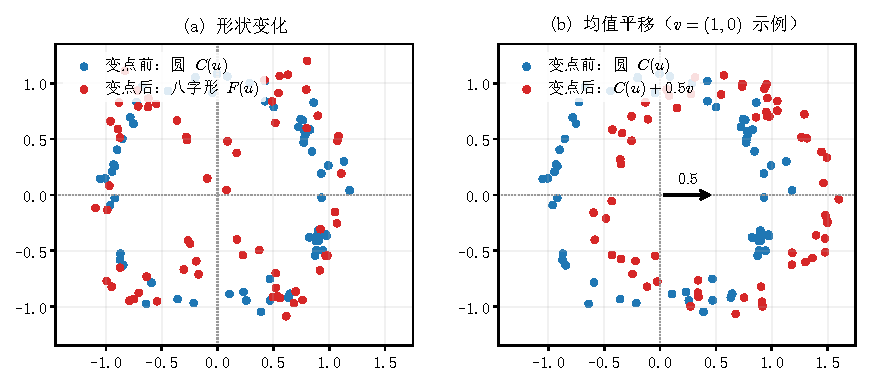
\includegraphics[width=0.90\textwidth]{../artifacts/figures/FigureA_alternative_geometry_short.pdf}
\caption{圆—八字形变化与整体平移备择的点云示意}
\label{fig:alternatives}
\caption*{\footnotesize 注：(a)圆形到八字形；(b)整体平移，示例方向 $v=(1,0)$。}
\end{figure}

\section{零假设下的有限样本校准结果}\label{sec:h0}

\subsection{拒绝率随步长的变化}\label{sec:h0-surface}
图~\ref{fig:bpi-h0}给出 BPI 在各条件下的经验拒绝率。固定窗口数时，M0 在 $s=8,16,32,64$ 下的范围依次为 $0.8816$--$0.9712$、$0.4384$--$0.7356$、$0.1088$--$0.3044$ 与 $0.0504$--$0.0528$；固定观测长度时，非重叠端（$s=64$）为 $0.0472$--$0.0608$。合并两种预算，BPI/M1 在 $s=8$ 时为 $0.0436$--$0.1180$，在 $s=64$ 时为 $0.0056$--$0.0276$。就全部 28 个配置而言，MOMENTS 的范围在 M0 下为 $0.0432$--$0.9996$、在 M1 下为 $0.0020$--$0.1412$。两种表示的 20 个唯一重叠配置中，M0 均被判为实质反保守；8 个非重叠配置中，M1 均被判为实质保守。全部 56 个匹配的“配置—表示”组合中 M1 的拒绝率都低于 M0，但降低拒绝率不能等同于恢复名义校准。

\begin{figure}[t]
\centering
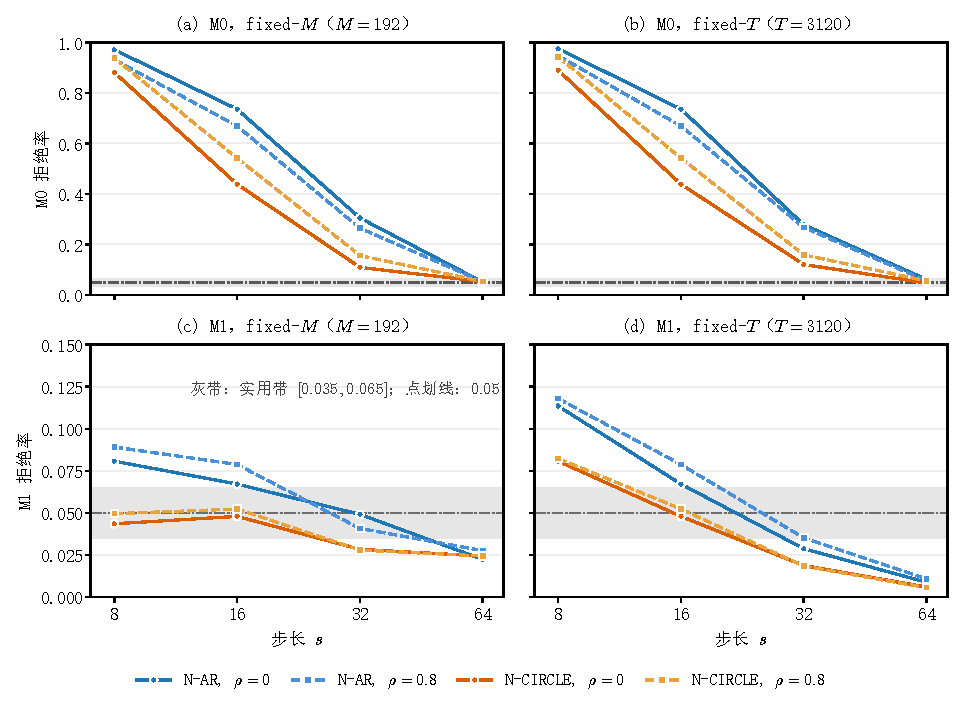
\includegraphics[width=0.96\textwidth]{../artifacts/figures/FigureB_BPI_H0_panels.pdf}
\caption{BPI 在两种预算制度与两种校准器下的零假设拒绝率（每格 $n=2500$）。(a)(b) 为 M0，纵轴 $[0,1]$；(c)(d) 为 M1，纵轴 $[0,0.15]$，两行量尺不同，曲线高度不可直接比较。灰带为实用等价带 $[0.035,0.065]$，点划线为名义水平 $0.05$；逐格分类仍依 Wilson 区间判据（\S\ref{sec:criteria}）。横轴为步长 $s$（对数刻度），连线只引导相邻设计点。实线/圆圈为 $\rho=0$，虚线/方块为 $\rho=0.8$；曲线未作平滑。}\label{fig:bpi-h0}
\end{figure}

\subsection{逐格校准分类}\label{sec:h0-classify}
112 个评价单元的四类计数见表~\ref{tab:calibration}。M0 在两种表示下均有 $20/28$ 个配置被判为实质反保守、没有配置被判为实质保守；M1 的分类分散于四类，说明依赖感知乘子改变了校准图谱的形态，却未实现统一校准。这些计数描述预设网格内的有限样本分布，不是方法在更广参数空间中的“通过率”。以固定窗口数、N-AR、$\rho=0$、BPI 为例，M0 在 $s=8,16,32$ 均为实质反保守、$s=64$ 转为实用校准；M1 随步长增加依次经历实质反保守、未定、实用校准与实质保守。这里报告的只是相邻格点的观测状态变化，不估计两点之间的连续临界步长（完整清单见补充材料 S1）。

\begin{table}[t]
\centering
\small
\caption{两种表示与两种校准方法的逐配置校准分类}\label{tab:calibration}
\begin{tabular}{llcccc}
\toprule
表示 & 方法 & 实用校准 & 实质保守 & 实质反保守 & 未定\\
\midrule
BPI & M0 & 7 (25.0) & 0 (0.0) & 20 (71.4) & 1 (3.6)\\
BPI & M1 & 5 (17.9) & 10 (35.7) & 7 (25.0) & 6 (21.4)\\
MOMENTS & M0 & 6 (21.4) & 0 (0.0) & 20 (71.4) & 2 (7.1)\\
MOMENTS & M1 & 1 (3.6) & 12 (42.9) & 7 (25.0) & 8 (28.6)\\
\bottomrule
\end{tabular}

\vspace{0.2em}
\begin{minipage}{0.95\textwidth}
\footnotesize 注：每行包含 28 个配置；括号内为百分比。分类判据见第~\ref{sec:criteria}~节。
\end{minipage}
\end{table}


\subsection{预设主对比}\label{sec:h0-primary}
表~\ref{tab:primary}报告 P1--P3 的点估计、边际 $95\%$ basic 自助区间与 Holm 校正结果。P1 与 P2 分别为 $0.5354$ 和 $0.5330$，区间下界均远高于预设阈值 $0.10$；P3 为 $0.0266$，区间整体高于 $0.01$，三项经 Holm 校正后 $p$ 均为 $0.00030$。因此，在两个预设数据生成过程、$\rho=0$ 与 BPI 表示的等权平均意义下，重叠端相对非重叠端的 M0 失校准超过 10 个百分点，且非重叠端的 M1 存在可检测的保守偏差；该结论不延伸为每一数据生成过程、依赖水平或表示下的必然规律。

对次级描述而言，原序列依赖对步长对比的修饰方向随生成过程与表示而异：$\rho$ 由 $0$ 变为 $0.8$ 时，$s=16$ 相对 $s=64$ 的拒绝率差异变化量介于 $-0.1148$ 与 $0.1032$ 之间，符号并不一致（定义与完整八值见 S7），故不提出依赖具有统一单调作用的结论。

\begin{table}[t]
\centering
\small
\caption{预设主对比 P1--P3 的效应估计与推断结果}\label{tab:primary}
\begin{tabular}{llccc}
\toprule
对比 & 估计量 & 点估计 & $95\%$ basic CI & Holm $p$\\
\midrule
P1 & fixed-$M$：$s{=}16$ 减 $s{=}64$（M0） & 0.5354 & $[0.5210,0.5494]$ & 0.00030\\
P2 & fixed-$T$：$s{=}16$ 减 $s{=}64$（M0） & 0.5330 & $[0.5194,0.5462]$ & 0.00030\\
P3 & $0.05$ 减 M1（$s{=}W{=}64$，fixed-$M$） & 0.0266 & $[0.0224,0.0308]$ & 0.00030\\
\bottomrule
\end{tabular}

\vspace{0.2em}
\begin{minipage}{0.95\textwidth}
\footnotesize 注：均针对 BPI 与 $\rho=0$，并对两个生成过程等权平均；区间为边际 $95\%$ 基本型自助置信区间，$p$ 为 Holm 调整后的单侧值。对比与阈值定义见第~\ref{sec:criteria}~节。
\end{minipage}
\end{table}


\section{表示的检出能力：形状变化与平移负对照}\label{sec:h1}

表~\ref{tab:h1}已完整报告两个场景的尺寸校正功效与场景差。形状变化下 BPI 的功效接近 $1$、MOMENTS 约 $0.06$，差异接近一个单位；平移负对照则正好反转，BPI 接近名义水平而 MOMENTS 接近 $1$，两个场景差的区间均不跨零。圆到八字形构造改变潜在几何并匹配单时点一、二阶矩；检出差异可能同时涉及连通、循环和度量几何变化，本实验未分离一维同调的贡献。

\begin{table}[H]
\centering
\small
\caption{两类备择下四个预设条件的等权尺寸校正功效与场景差（BPI 减 MOMENTS）。}\label{tab:h1}
\begin{tabular}{lccc}
\toprule
场景 & BPI 功效 & MOMENTS 功效 & 差值 $[95\%$ CI$]$\\
\midrule
形状变化 & 1.00000 & 0.06203 & $0.93797\ [0.92969,0.94609]$\\
均值平移 & 0.05375 & 1.00000 & $-0.94625\ [-0.95344,-0.93844]$\\
\bottomrule
\end{tabular}

\vspace{0.2em}
\begin{minipage}{0.95\textwidth}
\footnotesize 注：功效以各自匹配的零假设 $0.95$ 经验临界值计算；差值为两表示场景平均功效之差，其 $95\%$ 区间由 2000 次配对双层整簇自助法获得。逐条件的 nMAE、联合成功率与名义功效见补充材料 S7。
\end{minipage}
\end{table}


平移负对照有直接的结构解释。非重叠条件 $s=W=64$、$M=192$ 时 $T=12288$、$\tau=6144=96W$，变点恰落在第 96 与第 97 个窗口之间，没有窗口同时包含变化前后的观测；将 $H_1$ 与 $H_0$ 耦合到相同的潜变量与噪声路径时，每个后段窗口只是整体平移，故 $Y_{i,H_1}^{\mathrm{BPI}}=Y_{i,H_0}^{\mathrm{BPI}}$ 且 $T_{M,H_1}^{\mathrm{BPI}}=T_{M,H_0}^{\mathrm{BPI}}$。在该非重叠且边界对齐的构造中，BPI 统计量与匹配零假设具有相同分布，其检出概率等于匹配零假设下该经验临界值对应的拒绝概率；有限样本估计接近 $5\%$，但不要求精确等于 $0.05$，该结论对两种 $\rho$ 均成立。重叠条件 $s=16$、$M=192$ 时 $T=3120$、$\tau=1560$，只有第 95--98 号窗口跨越变点，其余窗口的 BPI 不变，故差异只能来自这些混合窗口。由于欧氏距离 Vietoris--Rips 构造对整体平移不变，该场景只能作为表示不变性的负对照，不能用于评价一般平移备择下的检出性能。

四个条件各 $1600$ 次重复；场景平均功效为 $1.00000$ 意味着四格估计均为 $1$，不构成总体功效恒等于 $1$ 的概率保证。定位与联合成功率见补充材料 S7：场景汇总的 nMAE 为 $0.00330$--$0.20255$，联合成功率为 $0.0009$--$0.9839$。本文不将其作为主贡献：位置误差由观测扫描曲线决定，校准方法只通过拒绝事件影响联合成功率，而失校准条件下的较高联合成功率可能部分来自过高的拒绝概率，须与匹配的零假设尺寸共同解释。

\section{讨论与结论}\label{sec:discussion}

窗口重用改变的是派生特征的联合分布，而不只是使有效样本量下降。即使原始观测独立同分布，重叠窗口仍会共享观测，派生特征因而可能相关；全局置换保留经验边际分布，却打散原顺序中的滞后协方差。命题~\ref{prop:counterexample}给出这种层级错配的有限样本反例，$3.974$ 只刻画标量窗口均值的方差比，不能外推为高维最大扫描的误报率倍数。因此，科学零假设成立不能自动提供窗口层面的排列不变性。

“降低误报”不等于校准。M1 在全部 56 个匹配组合中降低拒绝率，却在非重叠端系统保守、在强重叠端仍残留反保守；把方向相反的局部偏差汇总，可能得到接近 $0.05$ 的均值而掩盖严重失真，故逐格拒绝率与 Wilson 分类才是主要证据。表示敏感性与误报控制是两个维度：功效反转说明固定 BPI 保留了矩摘要未捕获的几何信息，但这既不能替代校准评价，也不能把全部检出优势归因于一维同调通道。

本研究的局限在于：结论限于固定 $W$、两个合成数据生成过程、固定 BPI 与 M1 配置、单变点最大扫描；未纳入自然数据、更多数据生成过程、多变点递归与表示超参数遍历；本文没有给出 BPI 扫描的通用有限样本定理，逐格分类为点态判据，M1 的带宽规则也未针对每个步长优化。对这些条件的推广需要新的理论与独立确认实验。


\section*{数据与代码可用性}
本文主稿、图件及补充材料 S1--S7 对应仓库 \url{https://github.com/dw0911/owtda-calibration} 中的标签 \texttt{short-202610-submission}（分支 \path{paper/short-202610}）。该版本提供代码、配置、随机种子及完整逐格结果；图表数据与生成说明见补充材料 S5。

\bibliographystyle{unsrt}
\bibliography{bibliography_short}
\end{document}
